\documentclass{article}\usepackage[]{graphicx}\usepackage[]{color}
%% maxwidth is the original width if it is less than linewidth
%% otherwise use linewidth (to make sure the graphics do not exceed the margin)
\makeatletter
\def\maxwidth{ %
  \ifdim\Gin@nat@width>\linewidth
    \linewidth
  \else
    \Gin@nat@width
  \fi
}
\makeatother

\definecolor{fgcolor}{rgb}{0.345, 0.345, 0.345}
\newcommand{\hlnum}[1]{\textcolor[rgb]{0.686,0.059,0.569}{#1}}%
\newcommand{\hlstr}[1]{\textcolor[rgb]{0.192,0.494,0.8}{#1}}%
\newcommand{\hlcom}[1]{\textcolor[rgb]{0.678,0.584,0.686}{\textit{#1}}}%
\newcommand{\hlopt}[1]{\textcolor[rgb]{0,0,0}{#1}}%
\newcommand{\hlstd}[1]{\textcolor[rgb]{0.345,0.345,0.345}{#1}}%
\newcommand{\hlkwa}[1]{\textcolor[rgb]{0.161,0.373,0.58}{\textbf{#1}}}%
\newcommand{\hlkwb}[1]{\textcolor[rgb]{0.69,0.353,0.396}{#1}}%
\newcommand{\hlkwc}[1]{\textcolor[rgb]{0.333,0.667,0.333}{#1}}%
\newcommand{\hlkwd}[1]{\textcolor[rgb]{0.737,0.353,0.396}{\textbf{#1}}}%
\let\hlipl\hlkwb

\usepackage{framed}
\makeatletter
\newenvironment{kframe}{%
 \def\at@end@of@kframe{}%
 \ifinner\ifhmode%
  \def\at@end@of@kframe{\end{minipage}}%
  \begin{minipage}{\columnwidth}%
 \fi\fi%
 \def\FrameCommand##1{\hskip\@totalleftmargin \hskip-\fboxsep
 \colorbox{shadecolor}{##1}\hskip-\fboxsep
     % There is no \\@totalrightmargin, so:
     \hskip-\linewidth \hskip-\@totalleftmargin \hskip\columnwidth}%
 \MakeFramed {\advance\hsize-\width
   \@totalleftmargin\z@ \linewidth\hsize
   \@setminipage}}%
 {\par\unskip\endMakeFramed%
 \at@end@of@kframe}
\makeatother

\definecolor{shadecolor}{rgb}{.97, .97, .97}
\definecolor{messagecolor}{rgb}{0, 0, 0}
\definecolor{warningcolor}{rgb}{1, 0, 1}
\definecolor{errorcolor}{rgb}{1, 0, 0}
\newenvironment{knitrout}{}{} % an empty environment to be redefined in TeX

\usepackage{alltt}
%\usepackage{Sweave}
\usepackage{float}
\usepackage{graphicx}
\usepackage{tabularx}
\usepackage{siunitx}
\usepackage{mdframed}
\usepackage{geometry}
\usepackage{pdflscape}
\usepackage{natbib}
\bibliographystyle{..//refs/styles/besjournals.bst}
\usepackage[small]{caption}
\setkeys{Gin}{width=0.8\textwidth}
\setlength{\captionmargin}{30pt}
\setlength{\abovecaptionskip}{0pt}
\setlength{\belowcaptionskip}{10pt}
\topmargin -1.5cm        
\oddsidemargin -0.04cm   
\evensidemargin -0.04cm
\textwidth 16.59cm
\textheight 21.94cm 
%\pagestyle{empty} %comment if want page numbers
\parskip 7.2pt
\renewcommand{\baselinestretch}{1.5}
\parindent 0pt

\newmdenv[
  topline=true,
  bottomline=true,
  skipabove=\topsep,
  skipbelow=\topsep
]{siderules}

%% R Script


\IfFileExists{upquote.sty}{\usepackage{upquote}}{}
\begin{document}
\title{Rethinking False Spring Risk}
\author{Chamberlain, Wolkovich}
\date{\today}
\maketitle 

\renewcommand{\thetable}{\arabic{table}}
\renewcommand{\thefigure}{\arabic{figure}}
\renewcommand{\labelitemi}{$-$}
%%%%%%%%%%%%%%%%%%%%%%%%%%%%%%%%%%%%%%%%%%%%%%%%%%%%%%%%%%%%%%%%
\begin{center}
\LARGE\textbf{Tables and Figures}
\end{center}
\section{Determining Spring Onset}
\begin{figure}[H]
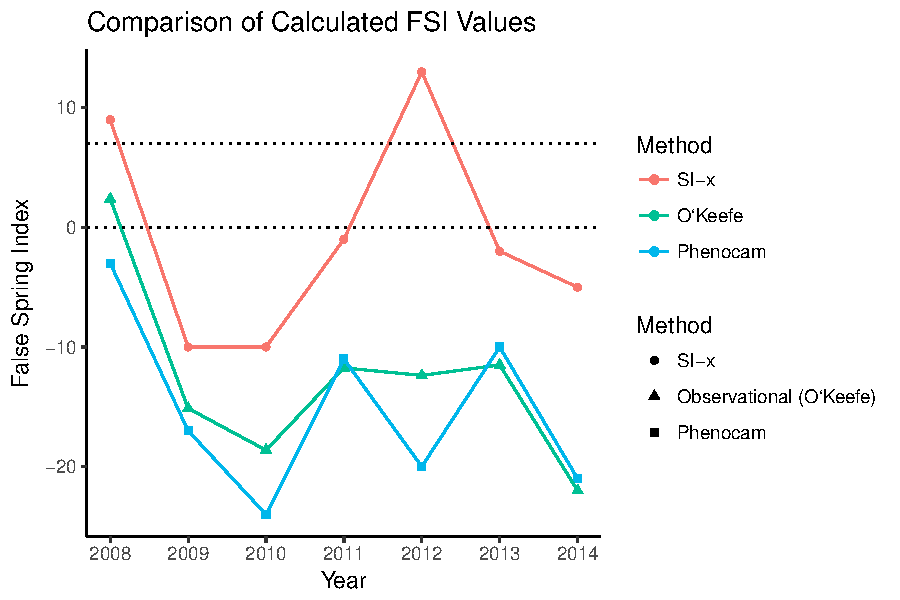
\includegraphics[width=\maxwidth]{figure/fsifig-1} \caption[A scatterplot indicating FSI values from 2008 to 2014 for each methdology used in this study]{A scatterplot indicating FSI values from 2008 to 2014 for each methdology used in this study. PhenoCam FSI values are red, Observed FSI values are blue, and USA-NPN FSI values are green.}\label{fig:fsifig}
\end{figure}



\section*{Species Differences and Vegetative Risk}
\subsection*{Treespotters Data}
\begin{figure} [H]
\begin{center}
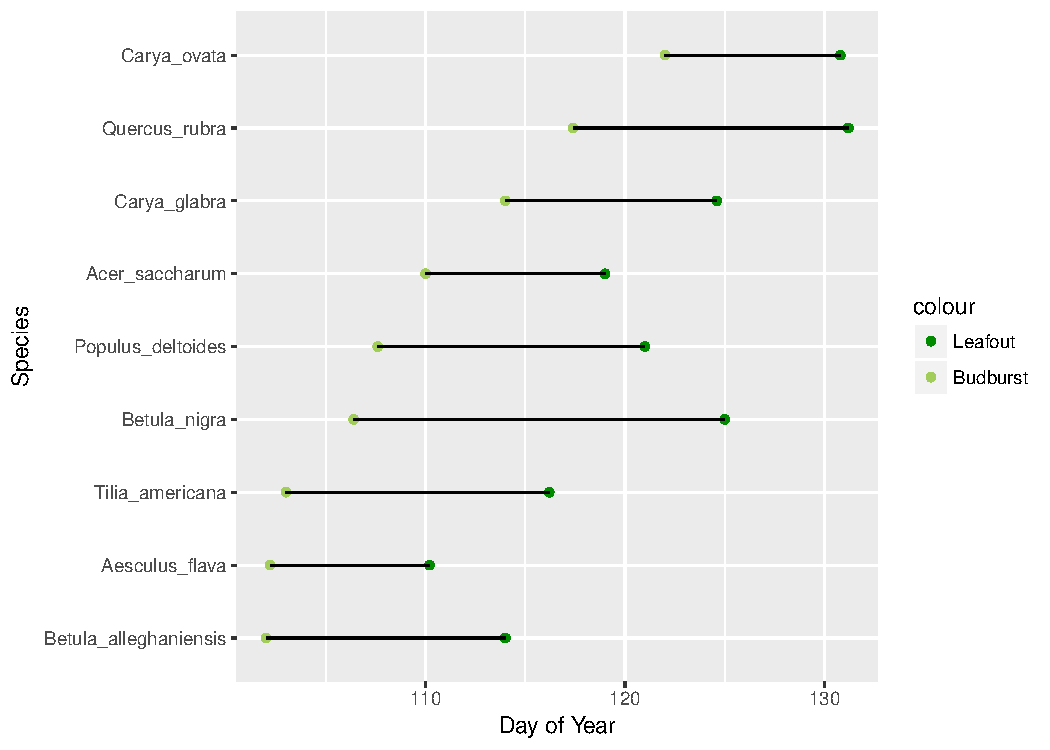
\includegraphics{..//figure/TreeSpot.pdf} 
\caption{Duration of vegetative risk for 9 native tree species in New England. Data was downloaded from the US-NPN data download tool (http://data.usanpn.org/observations/get-started) and observations were collected from the Arnold Aboretum - Tree Spotters program.  }
\end{center}
\end{figure}

% latex table generated in R 3.2.2 by xtable 1.8-2 package
% Tue Jun  6 15:36:42 2017
\begin{table}[ht]
\centering
\begin{tabular}{rrrrr}
  \hline
 & Estimate & Std. Error & t value & Pr($>$$|$t$|$) \\ 
  \hline
(Intercept) & 7.0456 & 9.4102 & 0.75 & 0.4575 \\ 
  Budburst & 0.0549 & 0.0858 & 0.64 & 0.5250 \\ 
   \hline
\end{tabular}
\end{table}


\subsection*{Dan's Data}
\begin{figure} [H]
\begin{center}
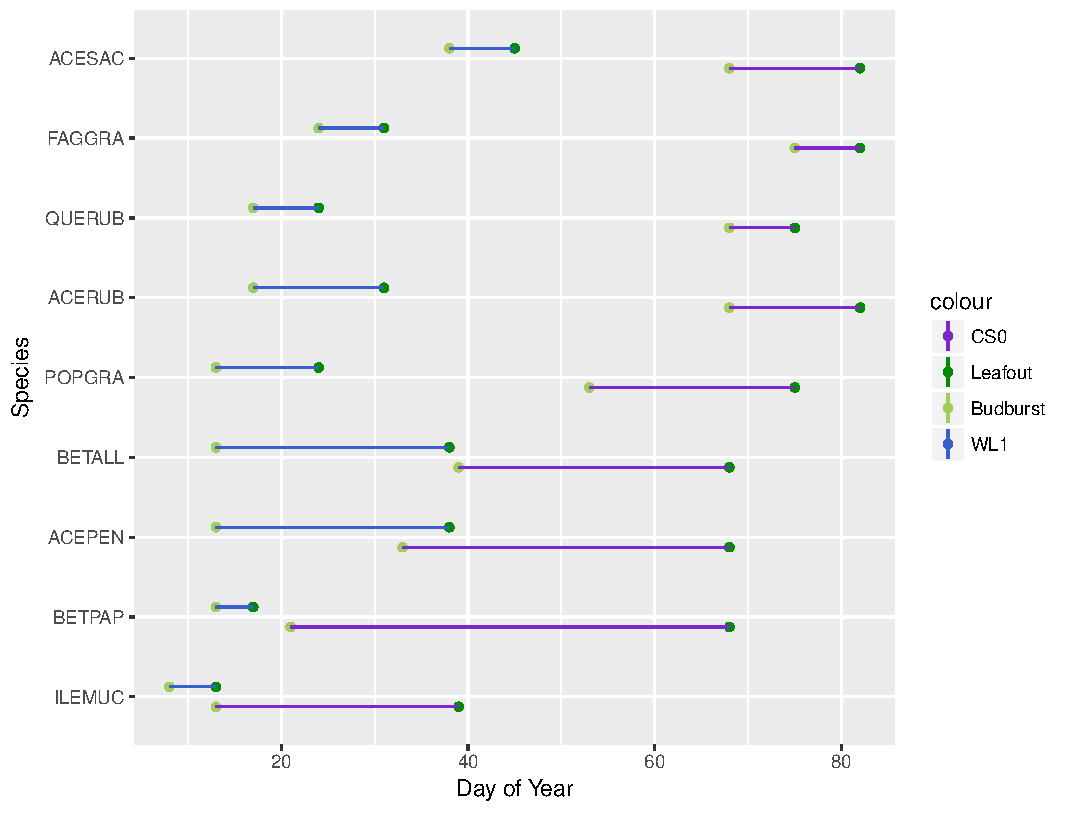
\includegraphics{..//figure/Exp_plot.pdf} 
\caption{Day of budburst and the day of leaf out for native tree species in New England. Data was collected from a growth chamber experiment using any combination of two photoperiod treatments, two forcing treatments, and three chilling treatments. The standard deviation is represented in blue for budburst and green for leaf out. }
\end{center}
\end{figure}


%<<label=expchill, results = "asis", echo=FALSE, fig.cap="The results from a linear regression model analyzing the relationship between latitude and frequency of false springs", fig.pos="H">>=
%read_chunk("..//scripts/anovas.R")
%d<-read.csv("..//input/Budburst.clean.csv",header=TRUE)

%dxx<-d
%dxx$chilling<- as.numeric(as.character(substr(dxx$chill, 6, 6)))
%dxx$warm<-as.numeric(as.character(dxx$warm))
%dxx$photo<-as.numeric(as.character(dxx$photo))
%dxx<-dxx %>%
  %dplyr::select(id, sp, site, lday, bday, chilling, warm, photo, treatcode)
%dxx$risk<-dxx$lday-dxx$bday 

%# Run anovas for each species
%myspp <- unique(dxx$sp)
%mylist<-list()
%for(i in c(1:length(myspp))) {
 % subby<-subset(dxx, sp==myspp[i])
  %myanova<-Anova(lm(risk~chilling + warm + photo, data=subby))
  %print(myanova)
  %mylist[[myspp[i]]] <- myanova
%}


%xtableList(mylist, title ="Anova results for Risk by chilling, forcing, and photoperiod effects for each species.")
%@

\subsection*{Harvard Forest Data}
\begin{figure}[H]
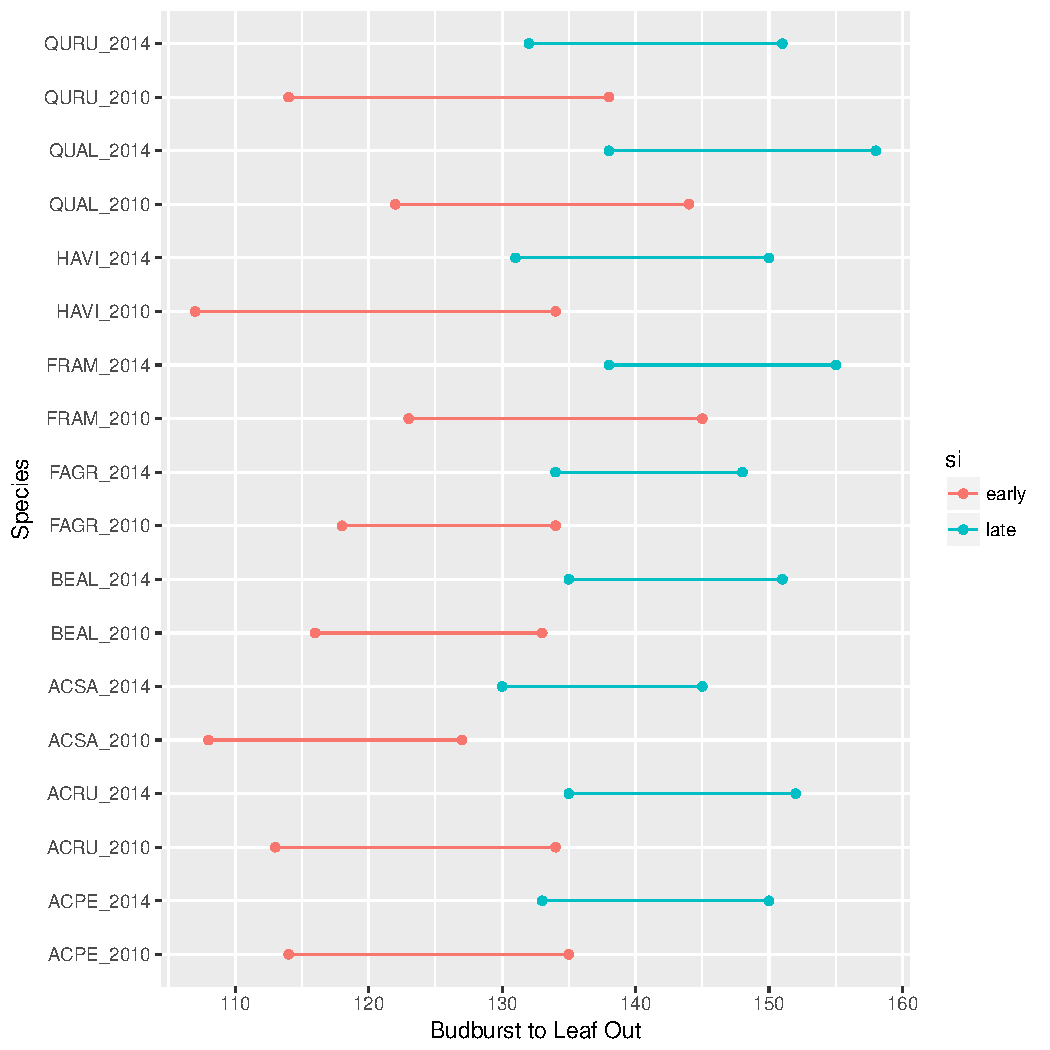
\includegraphics[width=\maxwidth]{figure/forest-1} \caption[A timeline plot indicating the duration of vegetative risk for each species from collected from Harvard Forest]{A timeline plot indicating the duration of vegetative risk for each species from collected from Harvard Forest.}\label{fig:forest}
\end{figure}


\section*{Regional Differences in Vegetative Risk?}
\begin{figure} [H]
\begin{center}
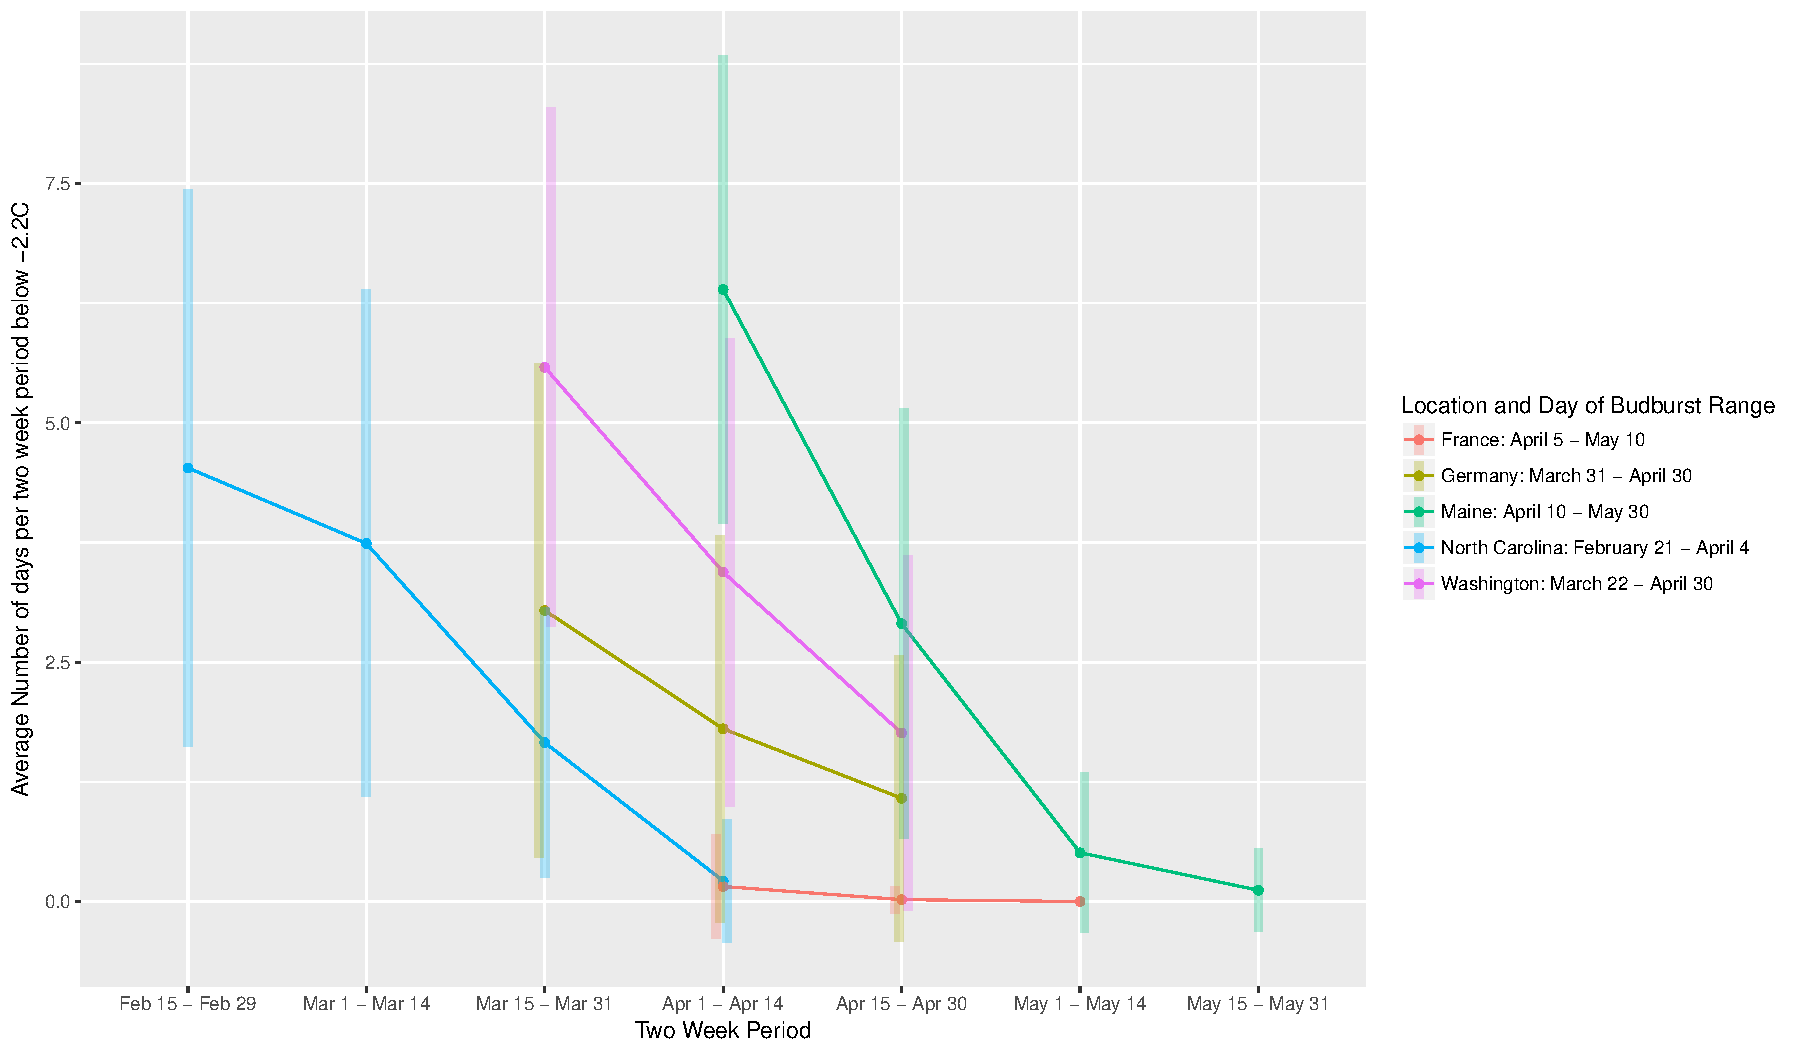
\includegraphics{..//figure/RegionalRisk_by_biweekly.pdf}
\includegraphics{..//figure/RegionalRisk_map.pdf}
\caption{Risk of a false spring event across five archetypal climate regions. The data was subsetted for each region based on earliest historical spring onset date to the latest historical leafout date and was divided into biweekly time periods \citep{SI-x2016, Soudani2012, Schaber2005}. We calculated the mean number of days that were -2.2$^{\circ}$C \citep{Ault2015, Schwartz2006, Schwartz1993} or below for each two week period that fell within the budburst to leafout timeframe in each region. }
\end{center}
\end{figure}

\section*{Temperature Thresholds for Damage: Agricultural vs Ecological}
\begin{landscape}
\begin{center}
\captionof{table}{Comparing damaging spring temperature thresholds in ecological and agronomical studies across various species and phenophases.} \label{tab:title} 
\footnotesize
\begin{tabular}{|c | c | c | c | c | c|}
\hline
\textbf{Sector} & \textbf{BBCH} & \textbf{Species} & \textbf{Temperature ($^{\circ}$C)} & \textbf{Type} & \textbf{Source} \\
\hline
Ecological & 9-15 & Sorbus aucuparia & -7.4 & 50\% lethality & \cite{Lenz2016} \\
\hline
Ecological & 9-15 & Prunus avium & -8.5 & 50\% lethality & \cite{Lenz2016} \\
\hline
Ecological & 9-15 & Tilia platyphyllos & -7.4 & 50\% lethality & \cite{Lenz2016} \\
\hline
Ecological & 9-15 & Acer pseudoplatanus & -6.7 & 50\% lethality & \cite{Lenz2016}\\
\hline
Ecological & 9-15 & Fagus sylvatica & -4.8 & 50\% lethality & \cite{Lenz2016}\\
\hline
Ecological & 9+ & All & -2.2 & hard & \cite{Schwartz1993}\\
\hline
Ecological & 9+ & All & -1.7 & soft & \cite{Augspurger2013} \\
\hline
Ecological & All & All & 2 SD below winter TAVG & cold-air outbreaks & \cite{Vavrus2006} \\
\hline
Ecological & 9+ & Eucalyptus pauciflora & -5.8 & elevated CO2 and temperature threshold & \cite{Barker2005} \\
\hline
Ecological & 9+ & All & -2.2 & 7 day threshold & \cite{Peterson2014} \\
\hline
Agrinomical & 9+ & All & 2 & Risk threshold for clear nights & \cite{Cannell1986} \\
\hline
Agrinomical & Floral & Vaccinium spp. & -4.4 to 0 & sprinkler protection threshold & \cite{Longstroth2012} \\
\hline
Agrinomical & 9 & Rosaceae & -7.2 & 10\% lethality & \cite{Longstroth2013}\\
\hline
Agrinomical & 9 & Rosaceae & -13.3 & 90\% lethality & \cite{Longstroth2013} \\
\hline
Agrinomical & All & All & Varies & Radiation Frost & \cite{Barlow2015} \\
\hline
Agrinomical & Floral & Wheat & -4 to -5 & 10-90\% lethality & \cite{Barlow2015} \\
\hline
Agrinomical & Vegetative & Wheat & -7 for 2hrs & 100\% lethality & \cite{Barlow2015} \\
\hline
Agrinomical & Vegetative & Rice & 4.7 & lethal limit & \cite{Sanchez2013} \\
\hline
Agrinomical & Vegetative & Corn & -1.8 & lethal limit & \cite{Sanchez2013}\\
\hline
Agrinomical & Vegetative & Wheat & -17.2 & lethal limit & \cite{Sanchez2013} \\
\hline
\end{tabular}
\end{center}
\end{landscape}
\restoregeometry



\section*{Conclusion - Box}
\captionsetup[table]{textformat=empty,labelformat=empty}
\captionof{table}{Key Indicators for Modeling False Spring Risk and Damage}
\begin{siderules}
\textbf {Box 1: Key Indicators for Modeling False Spring Risk and Damage}\\
In order to properly evaluate the expected level of damage sustained from a false spring event
key indicators should be included in the model.
\renewcommand{\theenumi}{\Roman{enumi}}
\renewcommand{\theenumii}{\roman{enumii}}
\scriptsize
\begin{enumerate}
  \item Life Stage of the Individual(s) \citep{Caffarra2011}
  \begin{enumerate}
    \item Seedlings and saplings will begin budburst earlier than adults
    \item The duration of vegetative risk may vary between life stages
    \item Long-term effects may vary
  \end{enumerate}
  \item Location Within a Forest \citep{Augspurger2013}
  \begin{enumerate}
    \item Individuals along the forest edge are more likely to experience a false spring
    \item Level of damage is likely to be higher at forest edges
  \end{enumerate}
  \item Amount of Winter Chilling (Flynn \& Wolkovich, 2017?)
  \begin{enumerate}
    \item Will affect the timing of budburst in the spring
    \item Will affect the duration of vegetative risk
  \end{enumerate}
  \item Proximity to Water %\citep{Gu2008}
  \begin{enumerate}
    \item Large bodies of water are expected to act as a buffer to spring freezes
  \end{enumerate}
  \item Precipitation Prior to Budburst \citep{Anderegg2013}
  \begin{enumerate}
    \item Will a drought increase cavitation and heighten damage from a false spring?
    \item Or will a drought decrease the risk of damage due to a lower chance of intracellular frost damage?
  \end{enumerate}
  \item Freeze Duration and Intensity
  \begin{enumerate}
    \item How should we define freezing temperatures?
    \item At what point is a freezing event severely damaging and xylem embolism occurs?
    \item How long must a false spring be to cause xylem embolism?
  \end{enumerate}
  \item Range of the Species
  \begin{enumerate}
    \item Species that have a more northern range may be more photoperiod than temperature sensitive 
  \end{enumerate}
\end{enumerate}
\end{siderules}

\bibliography{..//refs/SpringFreeze.bib}
\end{document}
